\documentclass[titlepage,a4paper,12pt]{report}
\usepackage{amssymb,amsfonts,amsmath}
\usepackage{fullpage}
\usepackage{graphicx}
%\usepackage[cc]{titlepic}
\usepackage{amsthm}
\newtheorem{definition}{Definition}[section]
\newtheorem{example}{Example}[section]
\newtheorem{theorem}{Theorem}[section]
\newtheorem{exercise}{Exercise}[section]
\newtheorem{corollary}{Corollary}[section]
\newtheorem{proposition}{Proposition}[section]
\pdfpagewidth 8.5in
\pdfpageheight 11in
\setlength\topmargin{-0.5in}
\setlength\headheight{0in}
\setlength\headsep{0in}
\setlength\textheight{9.5in}
\setlength\textwidth{7.0in}
\setlength\oddsidemargin{-0.5in}
\setlength\evensidemargin{1.0in}
\setlength\parindent{0.25in}
\setlength\parskip{0.25in}
%\begin{titlepage}
%\usepackage{titlepic}
%\titlepic{
\includegraphics[width=0.2\textwidth]{uz1.png}}
%
%\title{\textbf{HMTH111 Calculus 2}}
%\author{Nhawu. G\\
%		Department of Mathematics\\
%		University of Zimbabwe, ZIM}
%
%\end{titlepage}

\begin{document}
\begin{titlepage}
 
\begin{center}
 
 
% Upper part of the page

\includegraphics[width=0.15\textwidth]{uz1.png}\\[1cm]
 
\textsc{\LARGE University of Zimbabwe}\\[1.5cm]
 
\textsc{\Large HMTHCS111 CALCULUS 2}\\[0.5cm]
 
 
% Title

{ \huge \bfseries Calculus of Several Variables}\\[0.4cm]
 

 
% Author and supervisor
\begin{minipage}{0.4\textwidth}
\begin{center} \large
\emph{Author:}\\
G. \textsc{Nhawu}
\end{center}
\end{minipage}
\begin{minipage}{0.4\textwidth}
\begin{flushright} \large
\emph{Department:} \\
\textsc{Mathematics and Computational Sciences}
\end{flushright}
\end{minipage}

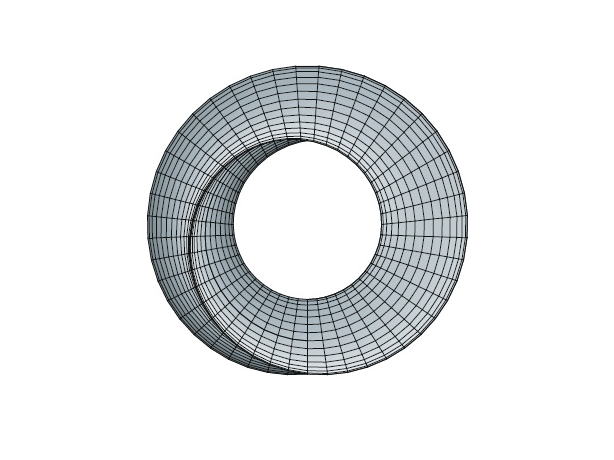
\includegraphics[width=0.7\textwidth]{umblictorus.png}\\[1cm]
 \vfill
 
 
% Bottom of the page
{\large \today}
 
\end{center}
 
\end{titlepage}
%\maketitle
%\tableofcontents
\begin{abstract}
\begin{center}
	\small{\parbox{18cm}{
		\begin{raggedright}
		{\small
		\textit{Everybody is a genius. But if you judge a fish by its ability to climb a tree, it will live its whole life believing that it is stupid.}
 }
 
				\vspace{.5cm}\hfill{---Albert Einstein}
		\end{raggedright}
	}
} 
\end{center}
These notes are not intended as a textbook. It is hoped however that they will minimize the amount of note-taking activity which occupies so much of a student’s class time in most courses in Mathematics. Probably the most important aspect of the notes is the set of tutorials. You should develop the practice of attempting several of these problems every week. Many of the problems are quite difficult so please consult your
tutor/lecturer if you are not blessed with success initially. Do not acquire the habit of abandoning a problem if it does not yield to your first attempt; a defeatist
attitude is your greatest adversary. Solution of a problem, even with some assistance
from the teacher when necessary, is a fine boost to your morale. You will find that a strong effort expended on the earlier part of the courses will be rewarded by growing
self-confidence and easier success later.

\noindent The emphasis is on understanding concepts. I think that nearly everybody agrees that
this should be the primary goal of calculus instruction. In fact, the impetus for the current
calculus reform movement came from the Tulane Conference in 1986, which formulated
as their first recommendation:
\begin{center}
\textit{Focus on conceptual understanding}.
\end{center}

\noindent I have tried to implement this goal through the \textit{Rule of Three}: ``Topics should be presented
geometrically, numerically, and algebraically.'' Visualization, numerical and graphical experimentation,
and other approaches have changed how we teach conceptual reasoning in fundamental
ways. The Rule of Three has been expanded to become the \textit{Rule of Four} by
emphasizing the verbal, or descriptive, point of view as well.
\end{abstract}
\chapter{What is Calculus?}
\begin{center}
	\small{\parbox{18cm}{
		\begin{raggedright}
		{\small
		\textit{A great discovery solves a great problem but there is a grain of discovery in the
solution of any problem. Your problem may be modest; but if it challenges your
curiosity and brings into play your inventive faculties, and if you solve it by your
own means, you may experience the tension and enjoy the triumph of discovery.}
 }
 
				\vspace{.5cm}\hfill{---George Poyla}
		\end{raggedright}
	}
} 
\end{center}
To a Roman in the days of the empire, a ``calculus'' was a pebble used in counting and
gambling. Centuries later, ``calculare'' came to mean ``to calculate,'' ``to compute,'' ``to
figure out.'' For our purposes, calculus is elementary mathematics (algebra, geometry,
trigonometry) enhanced by the \textit{limit process}.

\noindent It is fitting to say something about the history of calculus. The origins can be traced
back to ancient Greece. The ancient Greeks raised many questions (often paradoxical)
about tangents, motion, area, the infinitely small, the infinitely large, ---questions that
today are clarified and answered by calculus. Here and there the Greeks themselves
provided answers (some very elegant), but mostly they provided only questions.

\noindent After the Greeks, progress was slow. Communication was limited, and each scholar
was obliged to start almost from scratch. Over the centuries, some ingenious solutions
to calculus-type problems were devised, but no general techniques were put forth.
Progress was impeded by the lack of a convenient notation. Algebra, founded in the
ninth century by Arab scholars, was not fully systematized until the sixteenth century.
Then, in the seventeenth century, Descartes established analytic geometry, and the stage
was set.

\noindent The actual invention of calculus is credited to Sir Isaac Newton (1642-1727),
an Englishman, and to Gottfried Wilhelm Leibniz (1646-1716), a German. Newton's
invention is one of the few good turns that the great plague did mankind. The plague
forced the closing of Cambridge University in 1665, and young Isaac Newton of Trinity
College returned to his home in Lincolnshire for eighteen months of meditation, out
of which grew his method of fluxions, his theory of gravitation, and his theory of light.
The method of fluxions is what concerns us here. A treatise with this title was written
by Newton in 1672, but it remained unpublished until 1736, nine years after his death.
The new method (calculus to us) was first announced in 1687, but in vague general
terms without symbolism, formulas, or applications. Newton himself seemed reluctant
to publish anything tangible about his new method, and it is not surprising that its
development on the Continent, in spite of a late start, soon overtook Newton and went
beyond him.

\noindent Leibniz started his work in 1673, eight years after Newton. In 1675 he initiated the
basic modern notation: $dx$ and$\int$. His first publications appeared in 1684 and 1686. These
made little stir in Germany, but the two brothers Bernoulli of Basel (Switzerland) took
up the ideas and added profusely to them. From 1690 onward, calculus grew rapidly and
reached roughly its present state in about a hundred years. Certain theoretical subtleties
were not fully resolved until the twentieth century.
\end{document}